\documentclass[11pt]{article}
\usepackage[a4paper,margin=1in]{geometry}
\usepackage{amsmath,amssymb,amsthm,mathtools}
\usepackage{booktabs}
\usepackage{enumitem}
\usepackage{graphicx}
\usepackage{microtype}
\usepackage{hyperref}
\usepackage[nameinlink,capitalise]{cleveref}
\usepackage[numbers,sort&compress]{natbib}

\newtheorem{theorem}{Theorem}[section]
\newtheorem{proposition}[theorem]{Proposition}
\newtheorem{corollary}[theorem]{Corollary}
\newtheorem{lemma}[theorem]{Lemma}
\theoremstyle{definition}
\newtheorem{definition}[theorem]{Definition}
\theoremstyle{remark}
\newtheorem{remark}[theorem]{Remark}
\newcommand{\norm}[1]{\left\lVert#1\right\rVert}
\newcommand{\tr}{\operatorname{tr}}
\newcommand{\Ran}{\operatorname{Ran}}
\newcommand{\E}{\mathcal E}

\title{Block Schur--Secular Contraction Budgets\\
\large Exact Threshold Geometry and a Four-Step Replacement for Pointwise Sub-Quarter Decay}
\author{Liang Wang}
\date{July 2026}

\begin{document}
\maketitle

\begin{abstract}
RH-90 certified a rank-one packet correction with contraction factor below
$0.24$ at one selected update in each of ten frozen channels.  RH-91 then
used pointwise sub-quarter contraction as a sufficient bootstrap hypothesis.
The present paper shows that this pointwise formulation is stronger than the
finite data support and replaces it by a block budget.

For an enriched Hermitian compression
\[
 H=\begin{pmatrix}A&b\\b^*&d\end{pmatrix},\qquad
 \Delta=d-\lambda_{\min}(H),
\]
and requested gain $\delta\ge0$, set
$M_\delta=A-(d-\delta)I$.  The exact threshold dichotomy is
\[
 \Delta\ge\delta
 \quad\Longleftrightarrow\quad
 \lambda_{\min}(M_\delta)\le0
 \quad\text{or}\quad
 \bigl(M_\delta\succ0\ \text{and}\ b^*M_\delta^{-1}b\ge\delta\bigr).
\]
In the coercive branch, every trial vector satisfies the defect identity
\[
 \Phi_\delta(x)=
 \delta-b^*M_\delta^{-1}b
 +(M_\delta x-b)^*M_\delta^{-1}(M_\delta x-b).
\]
Thus absolute Schur margins should be normalized by the requested gain, and
ill conditioning is separated from the final sign.

The variable-budget theorem allows one-step factors $\rho_j$ to vary and
requires only their block product to contract.  A 384-bit audit freezes four
exact rational factors in each channel.  All forty Schur forms are strictly
negative, every refreshed packet dominates its rank-one corrected
predecessor, and the largest four-step budget is
$0.003219969564<0.24^4$, with geometric mean $0.23821162$.  Conversely,
seven individual updates have a positive-definite $0.24$ threshold matrix;
the smallest obstructed contraction is $0.25042832$.  Hence the block law is
genuinely weaker than pointwise sub-quarter decay.

This is an exact finite-dimensional reduction and a frozen four-step
certificate, not a repeated all-level block theorem.  Reduced packet refresh,
the prefix/observability bridge, Stage A, Hilbert--Polya, and the Riemann
Hypothesis remain open.
\end{abstract}

\noindent\textbf{Keywords:} Schur complement; secular equation; block
contraction; Rayleigh--Ritz; validated numerics; dynamic packet.

\medskip
\noindent\textbf{MSC 2020:} 47A75; 15A18; 65F15; 65G20; 37C30.

\section{Introduction}

The normalized-memory packet route replaces unstable tail eigenspaces by
captured energy.  RH-86 introduced the trace-normalized memory Gramian
\citep{WangMemory2026}; RH-89 showed that one complement direction and an
$(r+1)$-dimensional Ritz solve recover most of the observed reoptimization
dividend \citep{WangRitz2026}; and RH-90 removed the full reference packet
from a selected one-step certificate \citep{WangSchur2026}.  RH-91 then
isolated a sufficient all-level hypothesis: after burn-in, every update
contracts the memory tail by a fixed factor $\rho<1$
\citep{WangPacketReview2026}.

The first purpose of this paper is to sharpen the algebra behind that
hypothesis.  The RH-90 trial inequality is sufficient, but the compressed
matrix admits an exact necessary-and-sufficient dichotomy.  Either the old
block already contains a threshold direction, or a positive-definite
resolvent-weighted coupling must cross the requested gain.  Completing the
square then gives an exact trial-defect identity.  These statements identify
the natural relative margin and explain why a tiny absolute value of
$\Phi_\delta$ need not signal a fragile mechanism.

The second purpose is structural.  Uniform pointwise contraction is often
stronger than decay of a nonautonomous product.  For positive tails, the
quantity that enters a multi-update bootstrap is
$\prod_j\rho_j$, not $\max_j\rho_j$.  We therefore replace a fixed one-step
target by a variable contraction budget and prove a block bootstrap with an
explicit within-block prefix constant.  The proof is elementary, but the
change of quantifier is important: intermittent slow updates are permitted
provided the block has enough compensating decay.

The third purpose is a validated route audit.  We examine the four updates
ending at the archived packet time (with a one-step adjustment at the
coarsest scale).  The result has both positive and negative parts:

\begin{enumerate}[leftmargin=2em]
\item all forty variable-budget Schur gates are strict and all ten four-step
products lie below $0.24^4$;
\item seven of the same updates rigorously fail the pointwise $0.24$ target
for the named rank-one compressed correction;
\item a refreshed leading packet is no worse than the small corrected packet
at all forty steps, but producing such a refresh in polylogarithmic dimension
remains a separate theorem gate.
\end{enumerate}

The last item prevents a common overinterpretation.  The block theorem does
not prove that repeatedly applying only one complement correction tracks the
optimal packet.  It assumes a refresh satisfying an energy dominance
inequality.  In the Stage-A dependency language, the block Schur law and the
reduced-refresh law remain distinct.

\section{Exact Schur threshold geometry}

Let $G\ge0$ be a finite-dimensional or trace-class Gram operator, let
$V:\mathbb C^r\to\mathcal K$ be an isometry, and let
$q\perp\Ran V$ be a unit complement direction.  Put $Z=[V,q]$ and
\[
 H=Z^*GZ=\begin{pmatrix}A&b\\b^*&d\end{pmatrix}.
\]
Retaining the leading $r$ eigenvectors of $H$ instead of the old coordinate
packet gains exactly
\begin{equation}
 \Delta=d-\lambda_{\min}(H)\ge0.
 \label{eq:gain}
\end{equation}
This is the one-dimensional deletion formula used in RH-90.  We now resolve
the threshold event $\Delta\ge\delta$ exactly.

\begin{theorem}[Exact Schur threshold dichotomy]
\label{thm:dichotomy}
For $\delta\ge0$, define
\[
 M_\delta=A-(d-\delta)I.
\]
Then
\begin{equation}
 \boxed{
 \Delta\ge\delta
 \iff
 \lambda_{\min}(M_\delta)\le0
 \quad\text{or}\quad
 \left(M_\delta\succ0\ \text{and}\
 b^*M_\delta^{-1}b\ge\delta\right).}
 \label{eq:dichotomy}
\end{equation}
In particular, a zero eigenvalue of $M_\delta$ already certifies the requested
gain; no pseudoinverse boundary case is needed.
\end{theorem}

\begin{proof}
Set $t=d-\delta$.  By \eqref{eq:gain},
$\Delta\ge\delta$ is equivalent to
$\lambda_{\min}(H)\le t$, hence to
\[
 \lambda_{\min}
 \begin{pmatrix}M_\delta&b\\b^*&\delta\end{pmatrix}
 \le0.
 \label{eq:threshold-matrix}
\]
If $\lambda_{\min}(M_\delta)\le0$, restricting the Rayleigh quotient to
vectors $(x,0)$ proves \eqref{eq:threshold-matrix}.  If
$M_\delta\succ0$, Schur congruence gives
\[
 \begin{pmatrix}I&-M_\delta^{-1}b\\0&1\end{pmatrix}^{\!*}
 \begin{pmatrix}M_\delta&b\\b^*&\delta\end{pmatrix}
 \begin{pmatrix}I&-M_\delta^{-1}b\\0&1\end{pmatrix}
 =
 \begin{pmatrix}
 M_\delta&0\\0&\delta-b^*M_\delta^{-1}b
 \end{pmatrix}.
\]
Sylvester inertia therefore proves the second branch and its converse
\citep{HornJohnson2013,Bhatia1997}.
\end{proof}

\begin{corollary}[Modal secular sum]
\label{cor:modal}
In the coercive branch, let
$M_\delta u_k=\mu_k u_k$ with $\mu_k>0$ and write
$\beta_k=u_k^*b$.  Then
\begin{equation}
 \Delta\ge\delta
 \iff
 \sum_{k=1}^r\frac{|\beta_k|^2}{\mu_k}\ge\delta.
 \label{eq:modal-sum}
\end{equation}
\end{corollary}

The weights in \eqref{eq:modal-sum} show why the raw cross norm
$\norm b^2$ is not the complete invariant.  Coupling to a weakly coercive
old-packet mode is amplified by $\mu_k^{-1}$.  Conversely, a large coupling
concentrated in stiff modes may be insufficient.

For a trial $x\in\mathbb C^r$, define the RH-90 quadratic
\begin{equation}
 \Phi_\delta(x)=x^*M_\delta x-2\operatorname{Re}(x^*b)+\delta.
 \label{eq:phi}
\end{equation}

\begin{proposition}[Coercive trial-defect identity]
\label{prop:defect}
If $M_\delta\succ0$ and $r_x=M_\delta x-b$, then
\begin{align}
 \Phi_\delta(x)
 &=\delta-b^*M_\delta^{-1}b
 +(x-M_\delta^{-1}b)^*M_\delta(x-M_\delta^{-1}b)
 \label{eq:complete-square}\\
 &=\delta-b^*M_\delta^{-1}b+r_x^*M_\delta^{-1}r_x.
 \label{eq:residual-defect}
\end{align}
Consequently, for $\delta>0$ and relative secular surplus
\[
 \kappa_\delta=\frac{b^*M_\delta^{-1}b}{\delta}-1,
\]
the trial sign is certified whenever
$r_x^*M_\delta^{-1}r_x\le\kappa_\delta\delta$.
\end{proposition}

\begin{proof}
Expand the square in \eqref{eq:complete-square}.  Substituting
$x-M_\delta^{-1}b=M_\delta^{-1}r_x$ gives
\eqref{eq:residual-defect}.
\end{proof}

This identity separates three effects.  The exact secular surplus is a
property of the compressed dynamics, the residual defect measures the trial
solve, and the absolute scale is $\delta$.  A Schur margin of order
$10^{-16}$ may therefore coexist with a meaningful relative surplus when the
requested gain is itself of order $10^{-13}$.  Ill conditioning can make the
trial difficult to discover, but once \eqref{eq:phi} is evaluated with a
strict sign, no inverse occurs in the final Rayleigh proof.  This distinction
is standard in validated linear algebra \citep{Higham2002,Rump2010}.

\section{Variable one-step budgets and block bootstrap}

For an isometric packet $V$, write
\[
 \E_G(V)=\tr G-\tr(V^*GV).
\]
Let $E>0$ be the tail assigned to the previous refresh packet and let
$C=\E_G(V)$ be its predictor tail in the new Gramian.  A target factor
$\rho\ge0$ requests gain
\begin{equation}
 \delta=C-\rho E.
 \label{eq:required}
\end{equation}
Unlike RH-90, we do not require the same $\rho$ at every update.

\begin{theorem}[Variable-budget correction and refresh]
\label{thm:variable-budget}
Let $U$ be the leading rank-$r$ Ritz packet in $\Ran[V,q]$, and let $P^+$ be
any rank-$r$ refresh packet satisfying
\begin{equation}
 \E_G(P^+)\le\E_G(U).
 \label{eq:refresh}
\end{equation}
Fix $\rho\ge0$ and define $\delta$ by \eqref{eq:required}.
If $\delta\le0$, the old packet already gives
$\E_G(P^+)\le C\le\rho E$.  If $\delta>0$ and either branch of
\cref{thm:dichotomy} holds, then
\begin{equation}
 \E_G(P^+)\le\E_G(U)=C-\Delta\le\rho E.
 \label{eq:one-step-budget}
\end{equation}
The same conclusion follows from any trial with
$\Phi_\delta(x)\le0$.
\end{theorem}

\begin{proof}
The old coordinate packet captures $\tr A$.  The leading rank-$r$ Ritz
packet captures
$\tr H-\lambda_{\min}(H)=\tr A+\Delta$, hence its tail is $C-\Delta$.
The dichotomy or trial inequality gives $\Delta\ge\delta$.  Insert
\eqref{eq:required} and then use \eqref{eq:refresh}.
\end{proof}

The refresh condition is deliberately stated as an energy inequality.  It
does not require a spectral gap or principal-angle estimate.  An exact
leading packet satisfies it by Ky Fan's principle, but a reduced algorithm
must prove it by some other means \citep{Parlett1998,GolubVanLoan2013}.

\begin{theorem}[Block contraction budget]
\label{thm:block}
Let $E_n\ge0$ be packet tails and suppose
\begin{equation}
 E_{n+1}\le\rho_{n+1}E_n,
 \qquad \rho_{n+1}\ge0.
 \label{eq:variable-recursion}
\end{equation}
Fix a block length $L$.  Assume that after a burn-in index $b$, every complete
block satisfies
\begin{align}
 \prod_{s=1}^L\rho_{b+kL+s}&\le Q<1,
 \label{eq:block-product}\\
 \max_{0\le t\le L}\prod_{s=1}^t\rho_{b+kL+s}&\le B
 \label{eq:prefix-product}
\end{align}
for all $k\ge0$, with the empty product equal to one.  Then
\begin{equation}
 E_{b+kL+t}\le BQ^kE_b,
 \qquad 0\le t\le L.
 \label{eq:block-tail}
\end{equation}
For the normalized memory Gramian with parameter $0\le\eta<1$,
$E_b\le(1-\eta)^{-1}$ and the current relative snapshot residual obeys
\begin{equation}
 \frac{\norm{X_{b+kL+t}(I-P_{b+kL+t})}_2}
 {\norm{X_{b+kL+t}}_2}
 \le \sqrt{\frac{BQ^k}{1-\eta}}.
 \label{eq:block-snapshot}
\end{equation}
\end{theorem}

\begin{proof}
Multiply \eqref{eq:variable-recursion} over $k$ complete blocks and then over
the first $t$ factors of the next block.  This gives
\eqref{eq:block-tail}.  Every normalized snapshot Gramian has trace one, so
the memory trace is at most $(1-\eta)^{-1}$.  The current snapshot is a
nonnegative weight-one summand of the memory residual, proving
\eqref{eq:block-snapshot}.
\end{proof}

\begin{corollary}[Four-step sub-quarter budget]
\label{cor:four-step}
If $L=4$, $Q\le0.24^4$, and $B=1$, then complete block endpoints have the same
average exponential rate as pointwise $0.24$ contraction.  At
$\eta=1/512$, the crude bootstrap reaches relative tolerances
$10^{-2},10^{-4},10^{-6},10^{-8},10^{-10},10^{-12}$ after respectively
$8,16,20,28,36,40$ updates.
\end{corollary}

The block endpoint count is rounded to a multiple of four.  It is not a claim
that the frozen four-step window repeats.  Establishing repeated blocks with
uniform $Q$ is the new analytic gate.

\section{Validated four-step audit}

\subsection{Frozen models, clocks, and windows}

We use the same five directional Gaussian models as RH-77--RH-91, with
\[
 \sigma\in\{0.16,0.08,0.04,0.02,0.01\},\qquad
 \eta=1/512,
\]
fine dimensions $32,64,128,256,512$, and clock ranks $4,5,6,6,7$.  If
$M_\sigma$ is the archived postblock horizon, the four-step window ends at
\[
 t_\sigma=\max\left\{4,\left\lceil\frac{2M_\sigma}{3}\right\rceil\right\}.
\]
Thus the audited windows are $1$--$4$, $3$--$6$, $8$--$11$, $14$--$17$,
and $19$--$22$ as the noise decreases.

At each update we form the previous leading packet, select the leading left
singular direction of the new cross block, solve the $(r+1)$-dimensional Ritz
problem, and then recompute a leading refresh packet.  The rank-one direction
is canonical for maximal one-direction cross coupling, but the theorem itself
uses only the resulting compression.

\subsection{Frozen rational budgets}

A binary64 pilot was used only to choose upward-rounded thousandths.  The
resulting integers were then frozen in the source file before the 384-bit
audit.  Each target is therefore the exact rational number
$\rho_j=n_j/1000$, and every block product is an exact rational product.
This target-selection/validation separation is important when the worst block
has only a few percent of product slack.

The factors need not be below $0.24$.  Seven are larger, with maximum
$0.753$.  All forty are below one, so the audited within-block prefix constant
is $B=1$.

\subsection{Three independent finite checks}

The audit uses three checks at every update.

First, the small compressed matrix and trial vector are lifted exactly from
their binary representations and $\Phi_\delta(x)$ is evaluated in Arb ball
arithmetic.  Thirty-nine trials use the coercive solve; one uses an explicit
negative direction of $M_\delta$.  The sign, rather than a floating inverse,
is the certificate.

Second, ambient residuals are evaluated by the metric-corrected identity
\begin{equation}
 \E_G(W)=\tr G-2\tr(W^*GW)
 +\tr\bigl((W^*W)(W^*GW)\bigr).
 \label{eq:metric-corrected}
\end{equation}
This is the exact energy of $(I-WW^*)$ for the lifted binary basis and remains
valid when $W^*W$ differs slightly from the identity.  We directly verify the
target contraction and the refresh dominance inequality.  The largest basis
orthogonality defect in the archive is below $2.24\times10^{-15}$.

Third, whenever the direct corrected contraction exceeds $0.24$, we form the
pointwise threshold matrix in \eqref{eq:threshold-matrix}.  Strict positivity
of every leading principal minor certifies positive definiteness by
Sylvester's criterion.  Hence the named compressed correction cannot meet the
pointwise target.  We archive both determinant lower bounds and the associated
positive pivots.

This three-layer design avoids conflating an almost orthonormal floating basis
with an exact isometry.  The Schur sign, ambient contraction, and refresh
dominance are each checked in their own frozen model.

\section{Results: seven slow steps, ten contracting blocks}

\begin{table}[ht]
\centering
\scriptsize
\begin{tabular}{rrrllrrr}
\toprule
$\sigma$ & side & rank & times & rational factors & budget mean & actual upper & slow steps\\
\midrule
0.16 & L & 4 & 1--4 & .010/.006/.004/.003 & .005180 & .004514 & 0\\
0.16 & R & 4 & 1--4 & .017/.007/.005/.003 & .006500 & .006109 & 0\\
0.08 & L & 5 & 3--6 & .014/.007/.009/.022 & .011802 & .010915 & 0\\
0.08 & R & 5 & 3--6 & .008/.048/.006/.009 & .012000 & .011628 & 0\\
0.04 & L & 6 & 8--11 & .219/.091/.064/.031 & .079297 & .078268 & 0\\
0.04 & R & 6 & 8--11 & .050/.099/.142/.059 & .080248 & .079692 & 0\\
0.02 & L & 6 & 14--17 & .753/.142/.126/.239 & .238212 & .237514 & 1\\
0.02 & R & 6 & 14--17 & .145/.277/.360/.120 & .204095 & .203851 & 2\\
0.01 & L & 7 & 19--22 & .336/.251/.169/.190 & .228120 & .227778 & 2\\
0.01 & R & 7 & 19--22 & .391/.251/.123/.156 & .208315 & .207707 & 2\\
\bottomrule
\end{tabular}
\caption{Four-step budgets.  ``Budget mean'' is the exact rational product to
the power $1/4$; ``actual upper'' is the interval upper bound for the product
of direct corrected contractions.  A slow step is one whose corrected
contraction is rigorously above $0.24$.}
\label{tab:blocks}
\end{table}

The hardest channel is the left channel at $\sigma=0.02$.  Its rational
budget product is
\[
 0.753\cdot0.142\cdot0.126\cdot0.239
 =0.003219969564
 =0.97052516\cdot0.24^4.
\]
The direct interval product is at most $0.003182397980$, with geometric mean
$0.23751368$.  The first step is much slower than $0.24$, but the next three
steps compensate.

\begin{table}[ht]
\centering
\small
\begin{tabular}{lr}
\toprule
validated quantity & worst certified value\\
\midrule
strict Schur signs & 40/40\\
refresh dominance inequalities & 40/40\\
pointwise $0.24$ positive-definite obstructions & 7\\
largest four-step budget mean & $0.2382116195$\\
largest direct four-step mean upper & $0.2375136767$\\
smallest coercive relative-surplus lower & $1.1169\times10^{-4}$\\
smallest absolute negative Schur margin & $7.3996\times10^{-18}$\\
largest trial-system condition number & $2.623\times10^{13}$\\
largest refresh/corrected tail ratio & $0.99996914$\\
smallest obstructed one-step contraction & $0.25042832$\\
smallest positive Sylvester pivot & $2.8254\times10^{-14}$\\
\bottomrule
\end{tabular}
\caption{Global 384-bit validation summary.  The relative-surplus lower bound
is obtained directly from the negative trial form and requested gain.}
\label{tab:validation}
\end{table}

The seven pointwise obstructions occur at
\[
 (0.02,L,14),\ (0.02,R,15),\ (0.02,R,16),
\]
and
\[
 (0.01,L,19),\ (0.01,L,20),\
 (0.01,R,19),\ (0.01,R,20).
\]
For each, the $0.24$ threshold matrix is strictly positive definite.  Thus
there is no trial vector hidden by a poor solve: the exact compressed gain is
below the requested pointwise gain.  This is a finite no-go result for the
named target, window, rank, and one-direction enrichment.  It is not a no-go
theorem for a different complement dimension, a different rank staircase, or
an eventual later-time regime.

\begin{figure}[ht]
\centering
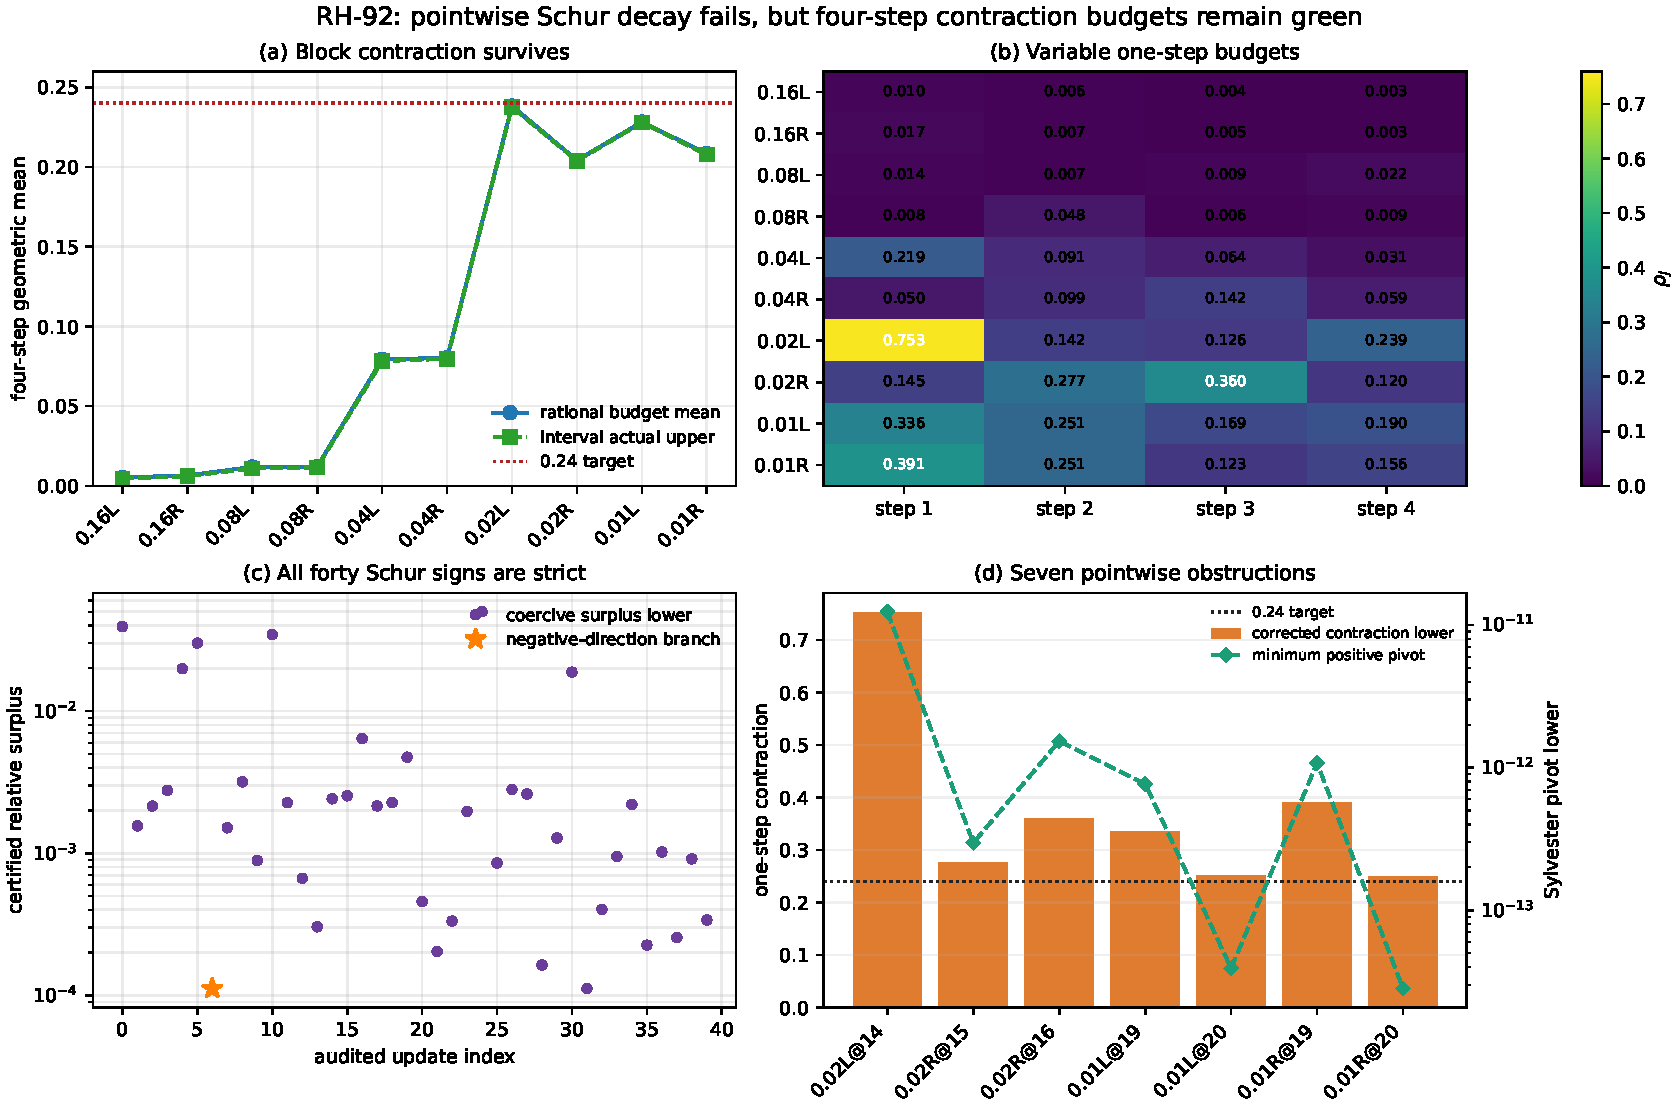
\includegraphics[width=\textwidth]{figures/block_schur_contraction_budgets.pdf}
\caption{The block budget versus the pointwise barrier.  Panel (a) shows that
all ten four-step geometric means remain below $0.24$.  Panel (b) displays the
exact rational factors.  Panel (c) gives certified relative Schur surplus
lower bounds, with the single negative-direction branch marked separately.
Panel (d) shows the seven pointwise obstructions and their positive Sylvester
pivots.}
\label{fig:audit}
\end{figure}

The refresh check is numerically close in one coarse update: the largest
refresh-to-corrected ratio is $0.99996914$.  It nevertheless remains strictly
below one at 384 bits.  At the fine scales the same ratio is generally farther
from one, but no uniform reduced-refresh theorem follows from these values.

\section{Route consequence and theorem boundary}

Let $L$ denote the inherited full-block corridor, $R$ the polylogarithmic
reduced packet refresh/future gate, and $O$ the finite-prefix,
normalization, and observability bridge.  RH-91 used $S_1$ for a pointwise
late Schur contraction law.  The present theorem shows that the sufficient
operator gate may instead be weakened to
\[
 S_{\mathrm{blk}}:
 \quad
 \prod_{s=1}^{L_0}\rho_{j+s}\le Q<1
 \quad\text{with a uniform finite prefix factor},
\]
for some fixed block length $L_0$.  The revised sufficient Stage-A formula is
therefore
\begin{equation}
 \mathsf A_1=L\ \vee\ (S_{\mathrm{blk}}\wedge R\wedge O).
 \label{eq:frontier}
\end{equation}
The frozen evidence suggests $L_0=4$ and $Q=0.24^4$, but does not prove that
choice uniformly.

This adjustment helps in two ways.  First, it removes seven artificial
one-step failures from the preferred corridor.  Second, the exact dichotomy
reduces each coercive update to the resolvent-weighted scalar
$b^*M_\delta^{-1}b/\delta$.  An all-level proof can now aim at an averaged
lower bound for secular surplus over four updates rather than a uniform
one-update lower bound.

It also sharpens what has \emph{not} been solved:

\begin{itemize}[leftmargin=2em]
\item Only one four-step window per frozen channel is certified.  Repetition
after an analytic burn-in remains open.
\item The rational factors are data-driven.  No formula bounds their product
from the continuum dynamics.
\item The audit refreshes with a leading ambient packet.  Replacing this by a
rank-$O(\log(1/\sigma))$ reduced future is exactly gate $R$.
\item The pointwise obstruction applies only to the named rank-one
enrichment.  It does not exclude a two-direction corrector or rank jump.
\item Gates $O$ and the RH-81 moving-cloud gates $P,C,U$ are unchanged
\citep{WangTwoCorridors2026,WangRouteReview2026}.
\end{itemize}

No canonical scattering completion, self-adjoint generator, intrinsic
$T\log T$ counting law, prime-power trace formula, completed-zeta identity,
Hilbert--Polya operator, zeta-zero identification, or proof of the Riemann
Hypothesis is obtained here.

\section{Reproducibility}

The archive contains the full and smoke audits, exact rational budget
manifest embedded in source, 384-bit interval records for all forty updates,
all Sylvester minors and pivots for the seven obstructions, the generated
figure, unit tests for the analytic formulas, and SHA-256 manifests for local
sources, external inputs, and publication artifacts.  The principal commands
are listed in the accompanying README.  All model matrices and trial vectors
are lifted from their binary representations; no decimal reconstruction is
used in a sign test.

\bibliographystyle{plainnat}
\bibliography{references}

\end{document}
